\documentclass[10pt,letterpaper]{article}
\setlength{\paperheight}{11in}
\setlength{\paperwidth}{8.5in}
\usepackage[ascii]{inputenc}
\usepackage{amsmath}
\usepackage{amsfonts}
\usepackage{amssymb}
\usepackage{graphicx}
\usepackage{gensymb}
\usepackage{enumitem}
\usepackage{float}
\usepackage{soul}
\usepackage{array}
\newcolumntype{C}[1]{>{\centering\arraybackslash}p{#1}}
\usepackage{latexsym}
\usepackage{chngpage}
\usepackage{hyperref} % Inserts hyper-references in the table of contents
\hypersetup{
	colorlinks,
	citecolor=black,
	filecolor=black,
	linkcolor=black,
	urlcolor=black
}
\usepackage{tikz} 			% Diagrams
\usetikzlibrary{arrows}		% Diagrams
\usepackage{verbatim}		% Diagrams
\tikzstyle{int}=[draw, fill=blue!20, minimum size=2em]
\tikzstyle{init} = [pin edge={to-,thin,black}]


\begin{document}
	
	% TITLE PAGE
	
	\begin{titlepage}
		\newcommand{\HRule}{\rule{\linewidth}{0.5mm}}
		\center
		
		\textsc{\LARGE McMaster University}\\[1.5cm] % Name of your university/college
		\textsc{\Large System Design}\\[0.5cm] % Major heading such as course name
		\textsc{\large 4G06 Capstone Design Project}\\[0.5cm] % Minor heading such as course title
		
		\HRule \\[0.4cm] 
		{ \huge \bfseries OSTRICH \\[2mm] \textit{A Large Scale 3D Scanner}}\\[0.4cm] % Title of your document
		\HRule \\[1.5cm]
		
		\begin{tabular}{ccc}
			\bf{Paul Correia}		& \bf{Nicolas Lelievre} 	& \bf{Bennett Mackenzie}		\\
			Mechatronics Eng 		& Software Eng 				& Software Eng 					\\
			\textit{1132370} 		& \textit{1203446}			& \textit{1211985} 				\\ \\
			\bf{Tigran Martikian} 	& \bf{Balraj Shah} 			& \bf{Mykola Somov} 			\\
			Software Eng			& Software Eng				& Software Eng 					\\
			\textit{1213170} 		& \textit{1207997}			& \textit{1141160}
		\end{tabular}\\[4cm]
		
		{\large December 7, 2015}\\[3cm] 
		
		%\includegraphics{Logo}\\[1cm] % Include a department/university logo - this will require the graphicx package
		
		\vfill % Fill the rest of the page with whitespace
		
	\end{titlepage}
	
    
\thispagestyle{empty}

\tableofcontents


\newpage


\thispagestyle{empty}

\listoffigures

\listoftables


\newpage


\thispagestyle{empty}

\section*{Revisions}
\begin{center}
  \begin{tabular}{cccc}
      \hline 
      \sc{Revision} & \sc{Date} & \sc{Authors} & \sc{Description of Revision} \\ \hline
      0 & Dec 7, 2015 & $\begin{matrix} \text{Paul Correia} \\ \text{Nicolas Lelievre} \\ \text{Bennett Mackenzie} \\ \text{Tigran Martikian} \\ \text{Balraj Shah} \\ \text{Mykola Somov} \end{matrix}$ & Initial revision of the system design. 
  \end{tabular}
\end{center}

\newpage


\section{Introduction}
\subsection{System Purpose - CHANGE?}
The advent of three dimensional modeling has revealed many new possibilities in computer graphics used in a multitude of fields ranging from game design to medical applications. As of late, three dimensional scanners have become significantly more accessible to the average consumer and therefore have gained immense popularity among professionals and hobbyists alike. \par 
The main focus of scanning three dimensional objects has however remained transfixed on a relatively small scale, often within a human's reach. Although some hand held three dimensional scanners offer high resolution scans and very detailed renderings, they are limited to house-hold object sizes meaning that larger objects are not easily scanned using such methods. \par 
The goal of this project is to make large-scale three dimensional scanners more readily available to users in need of scanning objects larger than the average hand held scanner can accommodate as well as removing the human element required in scanning to ensure continuously accurate and autonomous scans. \par 
The purpose of this document is to specify the requirements necessary for this project in terms of a general system description as well as the system's capabilities, conditions and constraints. The document will be in continuous revision during the developmental cycle of the project and will aid in keeping requirements in a constant and clear focus.

\subsection{System Scope - CHANGE?}
The OSTRICH (\textit{Object Scanning Tetra Rotary Independent Copter Hybrid}) is the result of our autonomous large-scale three dimensional scanner. The scope of the project rests mostly on designing a functioning quad-copter capable of sustaining the weight of all instruments on board, as well as converting the gathered information into a three dimensional model and ensuring that the OSTRICH is autonomous enough to independently scan a large-sized object without necessary human intervention. Note however that some larger components of the project are outside of our scope and will therefore be adapted to function for our specific needs. \par 
Items of functionality that remain in scope are: 
\begin{enumerate}
	\item Designing a quad-copter capable of flight;
    \item Manipulating acquired flight controller to allow stable flight
    \item Manipulating basic object avoidance system to eliminate possible collisions;
    \item Designing a control system capable of automated flight and scans; 
    \item Designing a launchpad for distance and position locating as well as homing;
    \item Assembling basic 3D scanner capable of scanning objects within size limitations
    \item Interfacing with 3D model conversion software;
    \item Printing scans using a 3D printer;
\end{enumerate}
Items of functionality that remain outside of scope are:
\begin{enumerate}
	\item Designing a flight controller;
    \item Designing a collision avoidance system;
    \item Developing 3D model conversion software;
    \item Building a 3D printer;
\end{enumerate}
The goal of the OSTRICH is to be generally applicable to a wide range of possible uses for both professionals and hobbyists, depending on the intended applications. These may include surveying small buildings, rendering sculptures/statues, applications for entertainment such as game design or film, researching and studying fragile historical artifacts, and so on. 


\newpage


\subsection{Definitions, Acronyms \& Abbreviations - CHANGE?}
Below are definitions, acronyms and abbreviations for specific or uncommon words used in the following document. 
\begin{table}[ht]
  \begin{center}
    \begin{tabular}{p{4cm} p{8.5cm}}

        \textbf{3D} & In this context, the representation of a three dimensional real-world object in a two dimensional digital environment using geometric data. \\ \\
        
        \textbf{fps} & Camera's picture rate measured in \textit{frames per second}. \\ \\
        
        \textbf{MP} & A \textit{megapixel} refers to the size of an image in reference to a photo from a digital camera. \\ \\
        
        \textbf{Modular Component} & A component of the OSTRICH which is designed to be easily removable, repairable or replaceable. Most of the OSTRICH's outer hull constitutes as a Modular Component. \\ \\
        
        \textbf{Non-Modular Component} & A component of the OSTRICH which cannot be removed, replaced, or repaired with ease. \\ \\
        
        \textbf{ppi} & Camera's image resolution measured in \textit{pixels per inch}. \\ \\

        \textbf{Quad-copter} & A helicopter-like vehicle propelled by four rotors. In this context, it is relatively small and manageable by a single person. \\ \\

		% WTF?!?!?!?
        \textbf{OSTRICH} & Our project name abbreviation which stands for \textit{Object Scanning Tetra Rotary Independent Copter Hybrid}. \\ \\  % WTFFFFFFFFFFF

        \textcolor{red}{*} & A red asterisk denotes requirements that are liable to change during the development process.

    \end{tabular}
  \end{center}
\end{table}


\newpage


\subsection{References - CHANGE?}
\begin{enumerate}
	\item "Flying an Unmanned Aircraft for Work or Research." Government of Canada; Transport Canada; Safety and Security Group, Civil Aviation. Web. 2 Nov. 2015.
	\item "Advisory Circular (AC) No. 600-004." Government of Canada; Transport Canada; Safety and Security Group, Civil Aviation. 6 Jan. 2015. Web. 2 Nov. 2015.
\end{enumerate}


\newpage


\subsection{System Overview}

\subsubsection{Context Diagram - CHANGE?}
\begin{figure}[h]
\centering
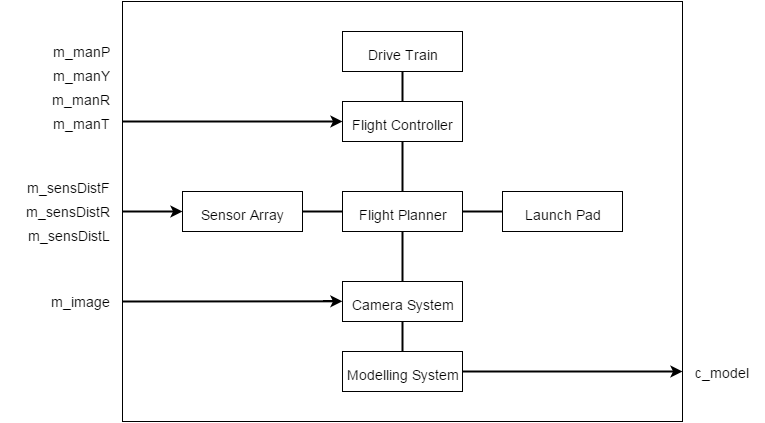
\includegraphics[scale=0.5]{Context_Diagram_1.png}
\caption{Context diagram for OSTRICH system}
\label{fig:context_diagram}
\end{figure}

\subsubsection{Component Diagram - PAUL}
Diagram showing components within system.

\newpage

\subsubsection{Monitored \& Controlled Variables - CHANGE?}
The monitor and control variables, as deemed necessary for the system to function properly according to system requirements, are listed in the below tables. \\

\begin{table}[H]
	\begin{center}
		\begin{tabular}{c p{6.5cm} cc}
        	\hline
            \sc{Variable} 	& \sc{Description} 	& \sc{Range} & \sc{Units} \\ \hline
            \texttt{m\_manP} & Manually controlled pitch (override) & 0 - 90 $\pm$ 5 & deg \\
            \texttt{m\_manR} & Manually controlled roll (override) & 0 - 90 $ \pm $ 5 & deg \\
            \texttt{m\_manY} & Manually controlled yaw (override) & 0 - 360 $ \pm $ 10 & deg \\
            \texttt{m\_manT} & Manually controlled thrust (override) & 0 - 0.5 $ \pm $ 0.05 & N \\
            \texttt{m\_Torq} & Torque produced from motors & 0 - x $ \pm $ y & N$\cdot $m \\
            \texttt{m\_DistR} & Distance from object on right & 0 - 6 $ \pm $ 0.1 & m \\
            \texttt{m\_DistL} & Distance from object on left & 0 - 6 $ \pm $ 0.1 & m \\
            \texttt{m\_DistF} & Distance from object in front & 0 - 6 $ \pm $ 0.1 & m \\
            \texttt{m\_PX}	& Position of the quad-copter on the x-axis & 0 - 10 $ \pm $ 0.2  & m \\
            \texttt{m\_PY} & Position of the quad-copter on the y-axis & 0 - 10 $ \pm $ 0.2 & m \\
            \texttt{m\_PZ} & Position of the quad-copter on the z-axis & 0 - 10 $ \pm $ 0.2 & m \\
            \texttt{m\_BatV} & Current battery voltage & 0 - 12 $ \pm $ 0.2 & V \\
            \texttt{m\_AnlgV} & Current Analog voltage & 0 - 5 $ \pm $ 0.2 & V \\
            \texttt{m\_BatI} & Current battery current & 0 - 25 $ \pm $ 0.2 & A \\
            \texttt{m\_Image} & Light reflection captured by camera & N/A & N/A \\
            \texttt{m\_CritS} & Critical Signal & 0 or 1 & Binary \\
            \texttt{m\_WarnS} & Warning Signal & 0 or 1 & Binary \\
		\end{tabular}
	\end{center}
\caption[Monitored System Variables]{Monitored System Variables}
\end{table}

\vspace{5mm}

\begin{table}[H]
	\begin{center}
		\begin{tabular}{c p{6.5cm} cc}
        	\hline
            \sc{Variable} 	& \sc{Description} 	& \sc{Range} & \sc{Units} \\ \hline
            \texttt{c\_Pitch} & Tilting about the x-axis & 0 - 90 $ \pm $ 5 & deg \\
            \texttt{c\_Roll} & Tilting about the y-axis & 0 - 90 $ \pm $ 5 & deg \\
            \texttt{c\_Yaw} & Twist or oscillate about the z-axis & 0 - 360 $ \pm $ 10 & deg \\
            \texttt{c\_Thrust} & Upward thrust exerted by the motors & 0 - 0.5 $ \pm $ 0.05 & N \\
            \texttt{c\_CamIO} & Camera operation on or off & 0 or 1 & Binary \\
            \texttt{c\_State} & Current state of the system & N/A & Enum \\
            \texttt{c\_Timer} & Current timer count & 0 - $(2^{32}-1)$ & s \\
            \texttt{c\_OX} & Original position of quad-copter at the start of scan, x dimension. & 0-12 $ \pm $ 0.2 & s \\
            \texttt{c\_OY} & Original position of quad-copter at the start of scan, y dimension. & 0-12 $ \pm $ 0.2 & s \\
            \texttt{c\_ReferenceP} & Location of reference point. & N/A & m\\
         \end{tabular}
	\end{center}
\caption[Controlled System Variables]{Controlled System Variables}
\end{table}

\newpage 

\subsubsection{Constants - CHANGE?}
Constants relating to the system in order for it to function properly according to the requirements are listed in the below table.

\begin{table}[H]
	\begin{center}
		\begin{tabular}{c p{6.5cm} cc}
        	\hline
            \sc{Constant} 	& \sc{Description} 	& \sc{Value} & \sc{Units} \\ \hline
            \texttt{k\_FrameRate} & Frame rate of the camera & 1 & fps \\
            \texttt{k\_CamRes} & Camera resolution & 5 & MP \\
            \texttt{k\_TotalMass} & Mass of the OSTRICH  & 2\textcolor{red}{*} & kg \\
            \texttt{k\_TotalHeight} & Height of the OSTRICH & 20\textcolor{red}{*} & cm \\
            \texttt{k\_TotalWidth} & Width of the OSTRICH & 30\textcolor{red}{*} & cm \\
            \texttt{k\_TotalDepth} & Depth of the OSTRICH & 30\textcolor{red}{*} & cm \\
            \texttt{k\_Storage} & Maximum solid state storage capacity & 8\textcolor{red}{*} & GB \\
            \texttt{k\_MaxSpeed} & Maximum horizontal velocity of quad-copter & 1 & m/s\\
            \texttt{k\_DistTol} & Maximum positional error of a complete loop around scanning object & 0.05\textcolor{red}{*} & m\\
		\end{tabular}
	\end{center}
\caption[Constants of the System]{Constants of the System}
\end{table}


\newpage


\section{Behaviour Overview - NICK S}
The following section gives a brief overview of the behaviour of the OSTRICH its components within the context of completing its primary function of autonomously generating a 3D model. Within the following lists the bolded items will be the components being described.

\subsection{Hardware Components}
	\begin{enumerate}[label=\textbf{HC\arabic*}]
		\item The 4 \textbf{motors} will be used to provide flight for the quad-copter. There will be 3 analog signals that will trigger the motors to start and provide the torque needed to take off.\\
      
    	\item The \textbf{electronic speed controller} controls the speed and direction of the motor by converting incoming voltage  into an analog signal\\
    
    	\item The \textbf{battery} sends 11.1V to the system in order to power it.  \\
        
        \item The \textbf{flight controller} takes inputs for the thrust, pitch, yaw, and roll from a controller. This allows the system to respond to different flight paths.
        
        \item The \textbf{proximity sensor} will constantly detect distance to objects and alert when in danger of collision.
        
        \item The \textbf{camera module} takes usable pictures (no blur, high enough resolution, refer to Insight3D PDF).
        
        \item The \textbf{raspberry pi} acts as sufficient processing power to deal with scheduled tasks.
        
        \item The \textbf{storage} acts as sufficient storage volume for all images.
        
        \item The \textbf{reciever} accepts incoming signals from the transmitter, thereby controlling the quadcopter's movement.
        
        \item 
    
    \end{enumerate}


\newpage


\section{Component Analysis}
blurb

\subsection{Hardware}
blurb

\subsubsection{Motor - TIGRAN}
blurb
\begin{center}
  \begin{tabular}{r p{8.5cm}}
      \textbf{Input} & Three analog signals \\
      \textbf{Output} & m\_Torq \\
      \textbf{Behaviour} & The 4 motors will be used to provide flight for the quad-copter. There will be 3 analog signals that will trigger the motors to start and provide the torque needed to take off.\\
      \textbf{Timing} & N/A\\
  \end{tabular}
\end{center}

\subsubsection{Electronic Speed Controller - TIGRAN}
blurb
\begin{center}
  \begin{tabular}{r p{8.5cm}}
      \textbf{Input} & m\_AnlgV\\ & m\_BatV \\
      \textbf{Output} & 3 analog signals\\ & 5V DC voltage to power all electronics.\\
      \textbf{Behaviour} & The electronic speed controller controls the speed and direction of the motor by converting incoming voltage  into an analog signal.\\
      \textbf{Timing} & N/A\\
  \end{tabular}
\end{center}

\subsubsection{Battery System - TIGRAN}
blurb
\begin{center}
  \begin{tabular}{r p{8.5cm}}
      \textbf{Input} & mechanical switch\\ & relay signal \\
      \textbf{Output} & m\_BatV \\
      \textbf{Behaviour} & The battery sends 11.1V to the system in order to power it. \\
      \textbf{Timing} & The timing constraint for the battery system is the discharge time. When the battery reaches a low charge it will slowly bring the quad-copter down to a safe land.  \\
  \end{tabular}
\end{center}

\subsubsection{Flight Controller - TIGRAN}
\begin{center}
  \begin{tabular}{r p{8.5cm}}
      \textbf{Input} & m\_manT\\ & m\_manP\\ & m\_manY\\ & m\_manR \\
      \textbf{Output} & 4 analogue voltages for the ESCs \\
      \textbf{Behaviour} & The flight controller takes inputs for the thrust, pitch, yaw, and roll from a controller. This allows the system to respond to different flight paths. \\
      \textbf{Timing} & The timing constraint for the flight controller is the response time. The flight controller must respond with a reasonable set of time.\\
  \end{tabular}
\end{center}

\subsubsection{Proximity Sensor - BALRAJ}
blurb
\begin{center}
  \begin{tabular}{r p{8.5cm}}
      \textbf{Input} & m\_DistR\\ & m\_DistL \\& m\_DistF\\
      \textbf{Output} & 0-5V signal \\
      \textbf{Behaviour} & Will constantly detect distance to objects and alert when in danger of collision. \\
      \textbf{Timing} & Must be able to detect distance to objects fast enough as to avoid any collisions.  \\
  \end{tabular}
\end{center}

\subsubsection{Camera Module - BALRAJ}
blurb
\begin{center}
  \begin{tabular}{r p{8.5cm}}
      \textbf{Input} & m\_CamIO \\
      \textbf{Output} & m\_Image \\
      \textbf{Behaviour} & Take usable pictures (no blur, high enough resolution, refer to Insight3D PDF).  \\
      \textbf{Timing} & N/A\\
  \end{tabular}
\end{center}

\subsubsection{Raspberry Pi - BALRAJ}
blurb
\begin{center}
  \begin{tabular}{r p{8.5cm}}
      \textbf{Input} & m\_BatV \\ & m\_BatI\\ & c\_ReferenceP\\ & c\_CamIO \\
      \textbf{Output} & m\_CritS\\ & m\_WarnS\\ & c\_State\\& m\_Image \\
      \textbf{Behaviour} & Sufficient processing power to deal with scheduled tasks. \\
      \textbf{Timing} & Picture taking interval (must be able to finish with one image before the next one is taken), Must avoid race conditions with parallel processes. \\
  \end{tabular}
\end{center}

\subsubsection{Storage - BALRAJ}
blurb
\begin{center}
  \begin{tabular}{r p{8.5cm}}
      \textbf{Input} & m\_Image \\
      \textbf{Output} & m\_Image \\
      \textbf{Behaviour} & Must have sufficient storage volume for all images. \\
      \textbf{Timing} & Must save file before taking another picture. \\
  \end{tabular}
\end{center}

\subsubsection{Receiver - NICK L}
blurb
\begin{center}
  \begin{tabular}{r p{8.5cm}}
      \textbf{Input} & Radio signal \\
      \textbf{Output} & Flight controller input signals \\
      \textbf{Behaviour} & The receiver should accept incoming signals from the transmitter, thereby controlling the quadcopter's movement. \\
      \textbf{Timing} & Little to no latency or jitter. Latency, if present, must be consistent. \\
      \textbf{Performance} & The receiver must have sufficient range to not lose signal of the transmitter within an object of approved size.
  \end{tabular}
\end{center}

\subsubsection{Transmitter - NICK L}
blurb
\begin{center}
  \begin{tabular}{r p{8.5cm}}
      \textbf{Input} & Physical remote control switches \\
      \textbf{Output} & Radio signal fed into the receiver \\
      \textbf{Behaviour} & The transmitter should accept broadcast signals from the remote control to be received by the receiver, thereby manually controlling the quadcopter's movement. \\
      \textbf{Timing} & Little to no latency or jitter. Latecny, if present, must be consistent. \\
      \textbf{Performance} & The transmitter must broadcast a sufficient range so as to always reach the receiver on the quadcopter within an object of approved size.
  \end{tabular}
\end{center}

\subsubsection{Arduino - NICK L}
blurb
\begin{center}
  \begin{tabular}{r p{8.5cm}}
      \textbf{Input} & Proximity sensors \\
      & Raspberry Pi \\
      & Flight controller signals \\
      \textbf{Output} & Camera enable \\
      & Planned transmitter inputs \\
      \textbf{Behaviour} & The arduino must handle all flight planning and safety critical checks to ensure the quadcopter maneuvers predictably and safely around objects. \\
      \textbf{Timing} & Must pull information from sensors and calculate course of action fast enough to avoid unexpected/undesired behaviour. \\
      \textbf{Performance} & There must be sufficient processing power for scheduling of all necessary tasks.
  \end{tabular}
\end{center}

\subsubsection{Frame - NICK L}
blurb
\begin{center}
  \begin{tabular}{r p{8.5cm}}
      \textbf{Input} & N/A \\
      \textbf{Output} & N/A \\
      \textbf{Behaviour} & The quadcopter frame must securely contain, support and protect (to a reasonable degree) the components of the quadcopter. \\
      \textbf{Timing} & N/A \\
      \textbf{Performance} & Must hold all components and be sufficiently durable in order to not fail during flight.
  \end{tabular}
\end{center}


\subsection{Software}
blurb

\subsubsection{Arduino - TIGRAN}
blurb \\

\underline{\textit{Flight Planning}} \\[2mm]
blurb
\begin{center}
  \begin{tabular}{r p{8.5cm}}
      \textbf{Input} & sensor data \\ & state control data \\ & manual override \\
      \textbf{Output} & flight path\\
      \textbf{Behaviour} & Be able to plan all actions for the quad-copter.\\ 
      \textbf{Timing} & The timing constraint for flight planning is that it must run real-time. \\
  \end{tabular}
\end{center}

\underline{\textit{State Control}} \\[2mm]
blurb
\begin{center}
  \begin{tabular}{r p{8.5cm}}
      \textbf{Input} & check reference point\\ &  battery warning signal \\
      \textbf{Output} & current/next state \\
      \textbf{Behaviour} & All states must be covered for the system. It must be complete and disjoint. \\
      \textbf{Timing} & The timing constraint for the state control must be fast enough to avoid incorrect data / unexpected events. \\
  \end{tabular}
\end{center}


\subsubsection{Raspberry Pi - BALRAJ}
blurb \\

\underline{\textit{Battery Management System}} \\[2mm]
blurb
\begin{center}
  \begin{tabular}{r p{8.5cm}}
      \textbf{Input} & m\_BatV \\ & m\_BatI \\
      \textbf{Output} & m\_CritS \\ & m\_WarnS \\
      \textbf{Behaviour} & Accurately detect battery level. \\
      \textbf{Timing} & Sampling time should be fast enough to accurately detect if battery levels are getting low. \\
  \end{tabular}
\end{center}

\underline{\textit{Camera Control}} \\[2mm]
blurb
\begin{center}
  \begin{tabular}{r p{8.5cm}}
      \textbf{Input} & c\_CamIO \\
      \textbf{Output} & m\_Image \\
      \textbf{Behaviour} & Take enough pictures to accurately retrieve 3D Model. \\
      \textbf{Timing} & Timing between pictures should be evenly spread across whole process. \\
  \end{tabular}
\end{center}

\underline{\textit{Reference Point}} \\[2mm]
blurb
\begin{center}
  \begin{tabular}{r p{8.5cm}}
      \textbf{Input} & c\_ReferenceP \\
      \textbf{Output} & c\_State \\
      \textbf{Behaviour} & Able to locate reference point in an accurate and timely manner. \\
      \textbf{Timing} & Must be fast enough to avoid overshooting reference point. \\
  \end{tabular}
\end{center}


\subsubsection{Computer - NICK L}
blurb \\

\underline{\textit{3D Modelling Software}} \\[2mm]
blurb
\begin{center}
  \begin{tabular}{r p{8.5cm}}
      \textbf{Input} & Images \\
      \textbf{Output} & 3D model \\
      \textbf{Behaviour} & The 3D modelling software must convert images taken by the quadcopter during flight into an appropriate and accurate 3D model of the real-life object. \\
      \textbf{Timing} & The process should not surpass one hour. \\
      \textbf{Performance} & The output must be a distinguishable and useable 3D model.
  \end{tabular}
\end{center}

\underline{\textit{Modelling Controller}} \\[2mm]
blurb
\begin{center}
  \begin{tabular}{r p{8.5cm}}
      \textbf{Input} & Images \\
      \textbf{Output} & 3D modelling software script \\
      \textbf{Behaviour} & The  modelling controller will automate the use of all tools necessary to generate a 3D model from the images taken by the quadcopter in order to minimise the amount of human intervention. \\
      \textbf{Timing} & N/A \\
      \textbf{Performance} & Autonomously schedules tasks to render 3D model from pictures. 
  \end{tabular}
\end{center}


\newpage


\section{Normal Operation - NICK S}
this section details the Normal operation of individual components of the OSTRICH. For more information on the normal operational cycle of the entire OSTRICH system please see Draft System Requirements section 2 (General System Description).

\subsection{Normal Hardware Operation}
	\begin{enumerate}[label=\textbf{NH\arabic*}]
        \item The \textbf{Motors}, upon launch of the OSTRICH, will steadily increase in torque until the entire quad-copter steadily rises to a target height. Once at that height, the motors will maintain stability of the quad-copter as the various other components adjust voltage feeds to the motors to cause the quad-copter to move in an adequate manner to satisfy the OSTRICH's target flight planning. Once a landing sequence is initiated the motors will steadily lower their torque until the quad-copter comes to a safe landing.\\
      
    	\item The \textbf{Electronic Speed Controller} during operational sequence will intake a voltage and will output three modulated analogue signals which will controll and adjust the speed of the motors such that the OSTRICH can complete its operational flight path. \\
    
    	\item The \textbf{Battery} will output a voltage as long as the OSTRICH is powered on. This power is supplied to the rest of the system's hardware and is used to sustain the entire system.\\
        
        \item The \textbf{Flight Controller} takes in manual overide commands as well as its own readings to determine the state of the quad-copter. With this information, during normal operational sequence, the flight controller keeps the quad-copter stable enough to take satisfactory photos and steers it through its target flight path as detailed in its standard operational protocol.\\
        
        \item The \textbf{Proximity Sensors} constantly detect the distance from the sensor to the nearest object perpendicular to it, as long as the quad-copter is powered. The sensors then send the corresponding signals which result from this reading to the rest of the OSTRICH system.\\
        
        \item The \textbf{Camera Module} takes pictures during regular operational sequence at a constant predefined period. These phorots are stored onto the OSTRICH's storage.\\
        
        \item The \textbf{Raspberry Pi} reads various system critical readings at a regular period to determine the system's target state at all times when the system is executing its operational sequence.\\
        
        \item The \textbf{Storage} acts as storage space and as a transfer medium for all of the data that must be stored during any aspect of the OSTRICH's operation.\\
        
        \item The \textbf{Reciever} acts as a medium for the manual override and other external command signals to be recieved and then later registered by the rest of the OSTRICH platform.\\
        
        \item The \textbf{Transmitter} The transmitter is the manual human interface for interacting with the OSTRICH's manual overrides. If the OSTRICH is not powered, the transmitter will do nothing, and if it is powered any input through the reciever will override whatever inputs the OSTRICH may be recieving otherwise.\\
        
        \item The \textbf{Frame} acts as the skeleton of the quad-copter and keeps it as a single system at all times short of maintenance.\\    
	\end{enumerate}
    
\subsection{Normal Software Operation}
	\begin{enumerate}[label=\textbf{NS\arabic*}]
    
        \item The \textbf{Flight Planning} 
        	
        \item The \textbf{State Control}
        
        \item The \textbf{Battery Management System}
        
        \item The \textbf{Camera Control}
        
        \item The \textbf{Reference Point}
               
        \item The \textbf{3D Modeling Software}
        
        \item the \textbf{Modelling Controller}
        
    \end{enumerate}
    
    


\newpage


\section{Undesired Behaviour - BEN}
Currently, there are 9 defined undesired events for the system. What follows is a list of all undesired events and how they are handled.

\begin{enumerate}[label=\textbf{UB\arabic*}]
    
        \item \textbf{Sensors lose track of object} - Should the sensors lose the object (the sensors no longer can find the object), the quad-copter will perform emergency land operations.
        
        \item \textbf{Radio Interference}
        
        \item \textbf{Inclement Weather} - Though it is advised that in inclement weather the user NOT attempt to operate the system, if a user attempts to do so, the system will perform an emergency land operation. Inclement weather (wind) is determined by excessive disturbances to the system.
        
        \item \textbf{Low battery} - If the battery is low, the emergency land operation is performed to avoid risking damage to the quad-copter if the battery runs out mid-flight.
        
        \item \textbf{Malfunctioning Battery} - If the battery is malfunctioning , the system performs an emergency stop and all power to the battery is cut.
        
        \item \textbf{Malfunctioning sensor} - If the sensor readings are incorrect, or a sensor's value is jumping around too much, the system will perform the emergency land operation.
        
        \item \textbf{Unintended and Excessive Acceleration} - If excessive acceleration is occurring, i.e. the quad-copter is moving in excess of the limits specified in the requirements above a predefined margin for error, the system will attempt to perform emergency land.
        
        \item \textbf{Software Errors} - If an error is caught in the software that would cause a failure, instead the emergency land operation is performed.
        
        \item \textbf{Mechanical fault} - We pray.
        
        \item \textbf{No model produced} - The system will alert the user to attempt the operation again, and will provide the user with an error message indicating why the scan was unsuccessful (for example, object too small, too concave, etc.)
        
        \item \textbf{Emergency land cannot be performed} - If the system is hanging up and unable to perform emergency land, the system will come to a stop immediately in order to prevent any of the unintended events listed above that trigger emergency land from having negative consequences.
        
    \end{enumerate}




\newpage


\section{Items Likely to Change - CHANGE!}
This section will briefly explain all of the items in the requirements document that are more likely to change than anything else. All items that are considered "likely to change" are marked by a red asterisk throughout the document, and the rationale for these items will be listed here.\par

\begin{enumerate}
	\item Constants k\_TotalMass, k\_TotalHeight, k\_TotalWidth, k\_TotalDepth, and k\_Storage are deemed likely to change, as we have written preliminary values for said constants, but the actual hardware for the size of the OSTRICH's frame are liable to change based on testing.
    \item The scanning phase algorithm is also listed as likely to change. As testing is performed, it may be that to complete the scanning phase the algorithm will have to be modified.
    \item It is predicted that this is not a conclusive and final list of all system states, and that more distinct states may be deemed necessary as the system is designed.
    \item The launchpad and its implementation and use are things that are likely to change. Currently it functions as more or less a placeholder for a starting point for the launch, and a device through which to send instructions such as an emergency stop for the quad-copter.
\end {enumerate}


\end{document}